\chapter{TESS Light Curve Dataset}

\section{TESS Mission}

TESS (Transiting Exoplanet Survey Satellite) \parencite{Ricker2014} is a satellite launched by NASA in 2018.
While its primary mission is the discovery of exoplanets, TESS monitors all objects that exhibit signs of changing brightness, including variable stars.

The satellite is equipped with four 16 megapixel wide-field cameras, producing high-quality full-frame images.
Individual objects are then identified and target pixel files (TPFs) are created.

Light curves are then obtained by calculating flux from the TPFs for each object and assembling them into time-series, each data product is then given a unique TIC - a numerical identifier.\parencite{TESSDataProducts}


\begin{figure}[!htbp]
    \centering
    \includegraphics[width=0.7\linewidth]{images/05/tess_satellite}
    \caption[TESS Satellite]{The TESS satellite before its launch in 2018. \parencite{tess_satellite}}
    \label{fig:05_tess_satellite}
\end{figure}

\FloatBarrier


\section{Dataset}

Mgr.\,Marek Skarka\,Ph.D. (Astronomical Institute of the Czech Academy of Sciences) generously provided us with a cleaned subset of a manually labeled dataset from the northern TESS viewing zone, for full details concerning the original dataset see \cite{Skarka2022}.

\subsection{Classes}

The original dataset contains \textbf{3402} total light curves with various annotations.
In total, \textbf{49} different classes are present with only \textbf{13} having more than \textbf{10} samples.

The classes were then combined into \textbf{5} main superclasses.
Samples with multiple annotations spanning multiple superclasses like ROTM\slash ELL (Rotating\slash Eclipsing) or extremely rare classes like HB (\hyperref[item:02-horiozntal-branch]{Horizontal Branch star}) were discarded, since they constituted only a small fraction of the entire dataset (\textbf{55} samples), leaving \textbf{3347} light curves.

\begin{table}[H]
    \centering
    \footnotesize
    \renewcommand{\arraystretch}{1.1}
    \begin{tabularx}{\textwidth}{X c@{\hspace{3em}}c@{\hspace{3em}}c}
            \toprule
            \textbf{Class (Label)} & \textbf{Original Labels} & \textbf{Count} & \textbf{Total} \tabularnewline \midrule
            Non-Variable (\textbf{N}) & NONE & \num{1729} & \num{1729}   \tabularnewline \midrule
            Unspecified-Variable (\textbf{U})             & VAR & 720 & 720    \tabularnewline \midrule
            Pulsating (\textbf{P}) &
            \begin{tabular}{@{}c@{}}
                GDOR \\ DSCT+GDOR \\ GDOR+DSCT \\ DSCT
            \end{tabular} &
            \begin{tabular}{@{}c@{}}
                206 \\ 176 \\ 86 \\ 67
            \end{tabular} &
            535    \tabularnewline \midrule
            Rotating (\textbf{R}) &
            \begin{tabular}{@{}c@{}}
                ROTS \\ ROT \\ ROTM
            \end{tabular} &
            \begin{tabular}{@{}c@{}}
                175 \\ 74 \\ 13
            \end{tabular} &
            262    \tabularnewline \midrule
            Eclipsing (\textbf{E}) &
            \begin{tabular}{@{}c@{}}
                EA \\ ELL \\ EW \\ EB
            \end{tabular} &
            \begin{tabular}{@{}c@{}}
                47 \\ 24 \\ 17 \\ 13
            \end{tabular} &
            101    \tabularnewline \midrule
            Total & & & \num{3347} \tabularnewline
            \bottomrule
    \end{tabularx}
    \caption[TESS Dataset Classes]{The TESS light curve dataset with simplified labels.}
    \label{tab:05_base_class_counts}
\end{table}

\FloatBarrier

We provide a brief description of the original labels, full explanation is provided in the original article by~\cite{Skarka2022}.

\begin{itemize}
    \item \textbf{NONE} - Star shows no signs of variability.
    \item \textbf{VAR} - Star shows signs of variability, but the exact class couldn't be identified accurately.
    \item \textbf{CLASS} - Variability type as described in ~\hyperref[sec:02-variable-stars]{2.4 Variable Stars}, for example a \textbf{DSCT} annotation would refer to a ~\hyperref[subsubsec:02-dsct]{Delta Scuti} star.
    \item \textbf{CLASS1+CLASS2} - Combined class, shows mainly signs of the first class.
    \item \textbf{CLASS1/CLASS2} - Uncertain class, the star could be of either of the classes.
\end{itemize}

\subsection{Light Curves}

The light curves were recorded at a 2-minute cadence and have various lengths, ranging roughly from $\num{11000}$ to $\num{216000}$ observations.

In their raw form, the curves contain only a timestamp ($t$), flux measurement ($\Phi$) and error measurement ($\Phi_{err}$).
By default, TESS data products measure time in Barycentric TESS Julian Days (BTJD), with $\mathrm{BTJD} = 0$ corresponding to roughly midnight on 01/01/2015.

\begin{figure}[!htbp]
    \centering
    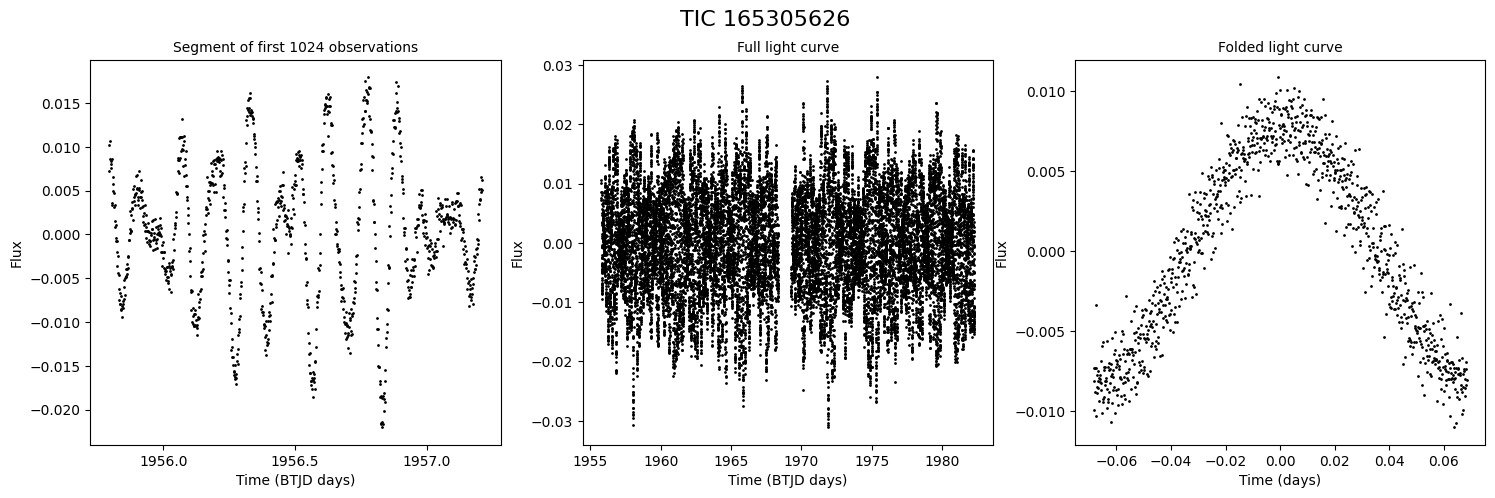
\includegraphics[width=\linewidth]{images/05_raw_light_curve}
    \caption[RAW Light Curve]{Raw light curve of a DSCT star, note the observation gap in the middle of the full light curve.}
    \label{fig:05_raw_light_curve}
\end{figure}

\FloatBarrier


\section{Preprocessing}

The original light curves were provided as a files in .csv format, each file representing a different light curve.

Raw light curves are not suitable for direct model ingestion due to their length, observation gaps and instrumental trends, additional preprocessing steps must therefore be taken to prepare the data.

Many different preprocessing approaches were tried and tested with different models producing various results, some of the preprocessing steps didn't yield any performance improvements and were therefore not used in the showcased models in the next chapter.
We therefore describe our approach of selecting appropriate preprocessing steps and extracting valuable information in the data while also discussing which preprocessing steps were unsuitable for the task.

\subsection{Time Standardization}

Since different light curves might have different starting times $t_0$, we need to remap the time axis to a common reference point, making the light curves comparable.
Zero was chosen as the time of the first observation, so all curves start at $t=0$.

\[
    t' = t - t_0
\]

\subsection{Flux Normalization}

Experiments have shown that the transformers perform better when the flux values are normalized, so we applied a modified \textbf{min-max normalization} to the \textbf{flux} ($\Phi$) values of each light curve.
The modified min-max normalization maps the flux values into range of $[-1, 1]$ instead of the more traditional range of $[0, 1]$, we have chosen this approach because it better represent the physical nature of the data where the flux oscillates above and below the zero centered norm.

\[
    \Phi' = 2 \cdot \frac{\Phi - \Phi_{\min}}{\Phi_{\max} - \Phi_{\min}} - 1
\]

We would like to add that experiments were performed with both mentioned types of normalization, however there were no measurable differences in predictive performance of the resulting models.

The normalization itself makes the various light curves comparable and allows for better generalization of the model, since the variability type is mainly distinguishable by the morphology of the light curve and not its amplitude.
The amplitude is extracted before normalization and stored as scalar value that can be utilized by combined models that are not strictly transformer based.

\subsection{Detrending}

Some form of detrending is often applied when preprocessing the light curves to remove instrumental noise, baseline drift and other low-frequency artifacts, however certain types of stars, particularly rotating variables, exhibit long-term patterns that are suppressed by the detrending algorithms.

Although multiple detrending algorithms were tried with various parameters, none of them yielded better results than the non-detrended original.

Flux detrending can be generally written as:

\[
    \Phi' = \Phi - \Phi_{\mathrm{trend}}
\]

Computation of $\Phi_{\mathrm{trend}}$ then depends on the detrending algorithm.

\subsubsection{Used Detrending Algorithms}

\begin{enumerate}
    \item \textbf{Running Median}
    \[
        \Phi_{\mathrm{trend}}(t_i) = \mathrm{median}\{\Phi(t_j): t_j \in [t_i - w/2, t_i + w/2]\}
    \]
    Where $w$ is the size of the sliding window where median is computed.
    \item \textbf{Gaussian Smoothing}
    \[
        \Phi_{\mathrm{trend}} = G(\Phi;\sigma)
    \]
    Where $G(\Phi;\sigma)$ represents a convolution of the flux $\Phi$ with a 1D gaussian kernel with standard deviation $\sigma$.
    \item \textbf{Polynomial Detrending}
    \[
        \Phi_{\mathrm{trend}} = p(\Phi)
    \]
    Where $p(\Phi)$ is a polynomial approximation of $\Phi$, usually low-order.
\end{enumerate}

While detrending still remains a valuable tool for many tasks (i.e.~searching for eclipsing binaries), its performance for our task proved insufficient and was therefore removed from the final pipeline.

\subsection{Observation Gaps}\label{subsec:05-observation-gaps}

Masking was used to handle observation gaps that are present in the data.
During preprocessing, all points with invalid flux values (NaN, +inf, -inf) are identified and a binary mask is constructed (True signals a valid position).

The mask is then applied during attention, preventing the invalid positions from influencing other tokens.
If a CLS token is used for classification, no other modifications are needed (since it was not influenced by the invalid positions), however when mean token pooling is used, the mask must be applied a second time to prevent the invalid tokens from being pooled alongside the valid ones.

\begin{figure}[!htbp]
    \centering
    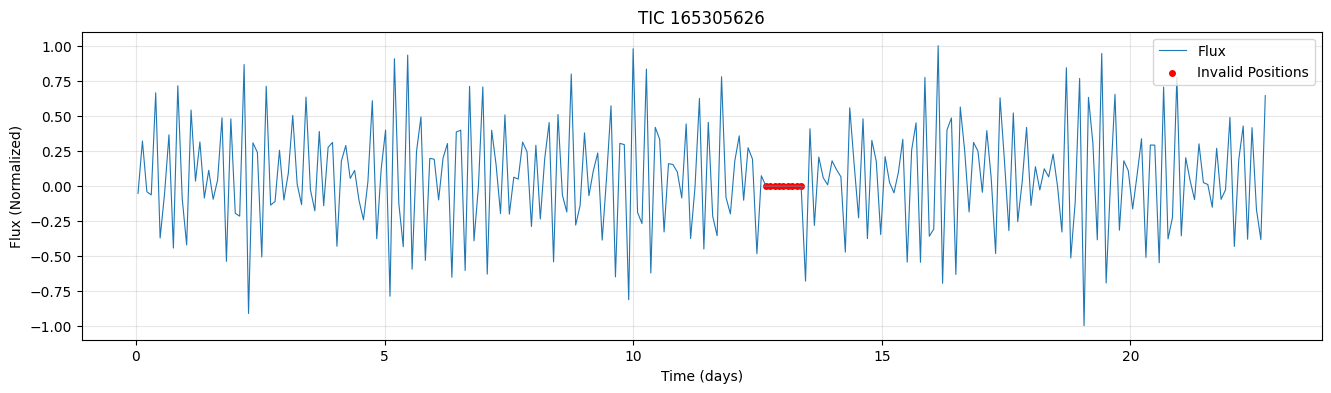
\includegraphics[width=\linewidth]{images/05/light_curve_invalid_positions}
    \caption[Observation Gap Masking]{A light curve with an identified observation gap (highlighted by red).}
    \label{fig:05_gap_masking}
\end{figure}

\FloatBarrier

\subsubsection{Handling Masks in Patch Embeddings}

When utilizing patch embeddings, additional measures must be taken to correctly apply the mask.

\subsection{Segmentation}

Since transformers have quadratic computation complexity with respect to the input sequence length \parencite{AttentionIsAllYouNeed}, feeding the entire light curves into the transformer quickly becomes infeasible\footnote{Training of a single-channel transformer on a dataset of $1000$ datapoints with length \num{4000} would take around $1$ minute per epoch. If a length \num{16000} (shortest light curves in the dataset) was used, the duration of one epoch would be roughly 16 minutes.}.
To address this issue, we tried various approaches that compact the light curves into more manageable form while preserving both local and global morphology.

\subsection{Multiple Time-domain Views}

As a solution to this problem, we propose providing the transformer model with multiple views of the given light curve, each having a different \textbf{temporal resolution}\footnote{Temporal resolution describes the amount of time that passes between observations - the measured flux ($\Phi$) values in our case. The default (highest) temporal resolution is 2-minutes in our dataset.}.
Multiple temporal resolutions allow us to capture periodic trends that are happening at different timescales while keep the individual views relatively short (our experiments have shown that $256$ is a good compromise of small size and high information content).

After several experiments, we decided to use the following 4 temporal resolutions for the views:

\begin{itemize}
    \item \textbf{2-minute resolution} (default)
    \item \textbf{8-minute resolution} ($\mathrm{bin\_size}=4$)
    \item \textbf{64-minute resolution} ($\mathrm{bin\_size}=16$)
    \item \textbf{128-minute resolution} ($\mathrm{bin\_size}=64$)
\end{itemize}

The views were then obtained by selecting an appropriate window from the light curve and mean-binning it to a specified fixed length that was same for all of the views.
For example, the 128-minute resolution view of size $256$ would be obtained by selecting a window of size

\[
    \frac{128 \, \mathrm{(resolution)}}{2 \, \mathrm{(default \, resolution)}} \cdot 256 \, \mathrm{(view \, size)} = \num{16384}
\]

then, mean-binning\footnote{The points are split into $n$ equally spaced, fixed-size bins ($n$ = 256, bin\_size = 64 in this case). A new sequence of length $n$ is then constructed where values at each position is the mean of all points in the corresponding bin.} the points in the window to length $256$ (size of $1$ bin would be $64$).

Each of the views starts at the beginning of the light curve / segment, this makes the smaller views subsequences of the larger views.
For example, assuming view size of $256$, the 2-minute resolution view becomes the first 4 points of the largest, lowest resolution 128-min view.

\begin{figure}[!htbp]
    \centering
    
\includegraphics[width=\linewidth]{images/05/light_curve_time_views}
    \caption[Multiple Time-domain Views]{An image showcasing 4 different time-domain views of a DSCT star's light curve. Each of the views contains $256$ data points which are sampled at $2$, $8$, $32$ and $128$ minute intervals respectively. A colored line shows an approximate position of each view in the original light curve.}
    \label{fig:05_light_curve_time_domain_views}
\end{figure}

\FloatBarrier

\subsubsection{Extracting Multiple Segments}

Another preprocessing method that greatly helped later models was the extraction of multiple segments from one light curve.
Since the dataset is quite small -- 898 light curves with specified variable class and only 101 of the class eclipsing -- the training of larger neural networks becomes difficult, especially when considering the predictive performance on marginalized classes.
This approach allowed us to partially overcome the size limitations of the dataset and utilize more information from each light curve.

The light curve was split into multiple segments, the size of each segment was equal to the size of the largest window.
Non-complete segments were also extracted, but they had to be masked similarly to the observation gaps, a minimum segment size was set in the pipeline as a hyperparameter.

The usage of segments brought multiple issues that needed to be resolved during training of the models, the solutions to these problems will be explained in more detail in the next chapter.

\begin{itemize}
    \item \textbf{TIC-level splitting.} To prevent leakage, the data were split into \linebreak train/val/test subsets based on a TIC (identifier of the light curve), therefore all segments from one light curve always ended in the same subset.
    \item \textbf{Segment Imbalance.} Since each light curve can have different number of segments, naive computation of class weights could throw off the trainer if one class had a very different average number of segments.
    \item \textbf{Evaluation.} A naive computation of evaluation metrics would not work well with multiple segments per light curve (example - what happens when out of 6 segments, 4 are predicted correctly and 2 incorrectly?).
\end{itemize}

\subsection{Phase-Folding}

A \hyperref[subsec:02-periodogram]{periodogram} was constructed using the Lomb-Scargle \parencite{Lomb1976} method, the top period was extracted and the light curve was \hyperref[subsec:02-phase-folded-light-curve]{phase-folded} accordingly.
The resulting phase-folded light curve was then binned to the required length.

\subsection{Feature Extraction}

Finally, additional features were extracted from each light curve and stored next to the sequences in the processed data.
These features can allow the model access to information that can't be easily extracted from the time-series.

\begin{itemize}
    \item \textbf{Amplitude.} Since the flux is normalized, amplitude introduces scale from the original light curve.
    \item \textbf{Top-10 Period.} 10 strongest periods identified in the periodogram.
    \item \textbf{Top-10 Powers.} Respective powers of the top-10 periods.
\end{itemize}

